\documentclass[number=01]{assignment}
\title{Computer Architecture - TE2031}
\chead{Tutorial}
\rhead{\ModelSim \& \Quartus enabling}


\newif\ifanswers
\answerstrue % comment out to hide answers

\newcommand{\deadline}{23:59 hours on Wednesday August 19th 2020.}

\newcommand{\SVcounterfile}{\colorfilename{counter.sv}}
\newcommand{\SVtbcounterfile}{\colorfilename{tb\_counter.sv}}

\newcommand{\SVdividefile}{\colorfilename{divide\_clk\_by\_2.sv}}
\newcommand{\SVtbdividefile}{\colorfilename{tb\_divide\_clk\_by\_2.sv}}

% Begin document
\begin{document}
\setcounter{chapter}{1}

\chapter*{Tutorial \\ \ModelSim \& \Quartus first time enabling}
\section{Objective}
\begin{itemize}
\item To enable \ModelSim and \Quartus software.
\item To understand the basics steps for compiling, simulating and synthesizing a \SV design using \ModelSim and \Quartus.
\end{itemize}

\section{Teamwork policy}
This is an individual assignment. 

\section{Background}
\ModelSim and \Quartus software are used for simulating, validating and synthesizing digital hardware designs using \acp{HDL}.
In this tutorial, you will refresh your knowledge on the basic use of these two tools. 

\section{Pre-requisites}
It is assumed that \ModelSim and \Quartus are installed in your computer.
If this is not the case, the attached document \colorfilename{ModelSim\_Quartus\_install.pdf} provides a quick guide on how to install these tools.
After you complete the installation of the tools, come back to this document and proceed with \sref{sec:ModelSim_project}.

\textbf{DISCLAIMER.} The versions of \ModelSim and \Quartus stated in the tutorial instructions \colorfilename{ModelSim\_Quartus\_install.pdf} are for reference only. 
You might find more recent versions of the software. However, the steps provided in this tutorial should still be relevant.
If you find a mistake in this tutorial due to a version update, please do let me know.
 
\newpage
% ======================================
% MODELSIM PROJECT
% ====================================== 
\section{\ModelSim project}\label{sec:ModelSim_project}
This section reinforces the steps necessary in order to create a \ModelSim project, compile and simulate a design.
If you are confident enough with your \ModelSim knowledge, you may skip \sref{sec:ModelSim_tutorial} and go straight to the exercise in \sref{sec:ModelSim_exercise}.

\subsection{Tutorial Instructions}\label{sec:ModelSim_tutorial}
  %\subsection{Creating a project}
  For this part of the tutorial, please use the source files \SVdividefile and \\\SVtbdividefile 
  \begin{enumerate}
    \item Open \ModelSim.
    \item From the top menu select \textbf{File} $\rightarrow$ \textbf{New} ${\rightarrow}$ \textbf{Project}
    \item Provide a name and a location for your project and click \textbf{OK}.
    You can select any project name you want. However, as shown in \fref{Figure:Project_name}, it is a good practice to match the name of your project with the name of your top-level \SV module. 
    %
    % Create project 
    %
    \begin{figure}[!htb]
    \centering
    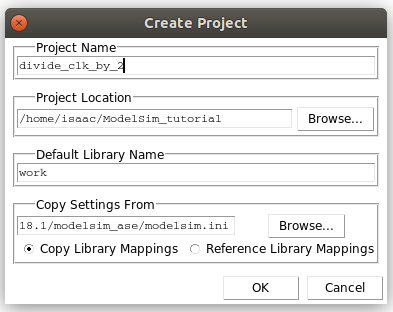
\includegraphics[scale=0.6]{ModelSim_tut_01}
    \caption{Project name and location.}
    \label{Figure:Project_name}
    \end{figure}
    %
    % Create project 
    %
    \item You should be prompted with the window shown in \fref{Figure:Add_files}.
    For this tutorial, you are provided with some \SV files, for this reason, select \textbf{Add Existing File}
    %
    % Add files
    %
    \begin{figure}[!htb]
    \centering
    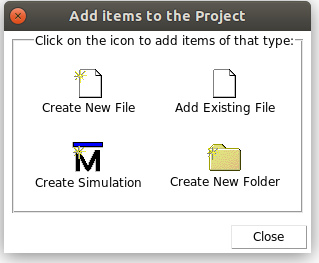
\includegraphics[scale=0.6]{ModelSim_tut_02}
    \caption{Add files prompt.}
    \label{Figure:Add_files}
    \end{figure}
    %
    % Add files
    %
    \item Browse to the location of the provided files for this tutorial, select \SVdividefile and \SVtbdividefile files and click \textbf{Open}. 
    As shown in \fref{Figure:Adding_files}, I've placed both files under the same location, which corresponds to the project's location. 
    However, this is not necessary and we can refer to files located elsewhere in our file system.
    %
    % Browse files
    %
    \begin{figure}[!htb]
    \centering
    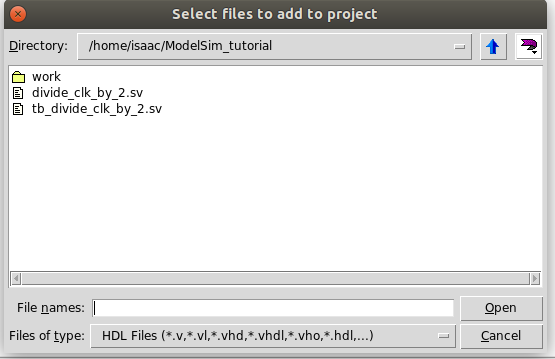
\includegraphics[scale=0.6]{ModelSim_tut_03}
    \caption{Files to be added.}
    \label{Figure:Adding_files}
    \end{figure}
    %
    % Browse files
    %
    \newpage
    \item As shown in~\fref{Figure:Add_files_OK}, make sure that \textbf{Reference from current location} is selected and select \textbf{OK}. 
    After this, you should see something similar to~\fref{Figure:Files_added}. 
    %
    % Add files OK
    %
    \begin{figure}[!ht]
    \centering
    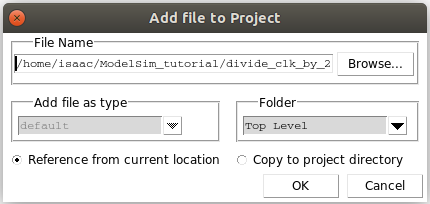
\includegraphics[scale=0.6]{ModelSim_tut_04}
    \caption{Adding project files.}
    \label{Figure:Add_files_OK}
    \end{figure}
    %
    % Add files OK
    %
    %
    % Added files
    %
    \begin{figure}[!ht]
    \centering
    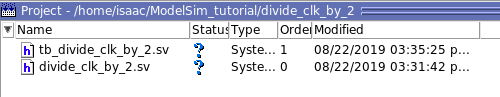
\includegraphics[scale=0.6]{ModelSim_tut_05}
    \caption{Files added to project.}
    \label{Figure:Files_added}
    \end{figure}
    %
    % Added files
    %
    \newline
    Note that there's a question mark (\textbf{?}) next to the name of the files. This indicates that the files have not been compiled since its creation or last modification.
    \newpage
\item In order to compile, select \textbf{Compile} $\rightarrow$ \textbf{Compile all} from the top menu.
As shown in \fref{Figure:Files_compiled1}, a green check mark next to the name of the file indicates a successful compilation. 
%
% Compiled files1
%
\begin{figure}[!htb]
\centering
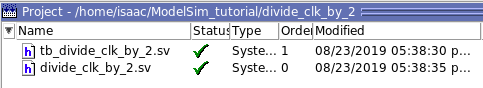
\includegraphics[scale=0.6]{ModelSim_tut_06}
\caption{Files compiled successfully.}
\label{Figure:Files_compiled1}
\end{figure}
%
% Compiled files1
%
\newline
\ModelSim also provides a command and message window, which is embedded in the bottom part of the screen. 
Here, \ModelSim also indicates if a compilation has been successful as shown in \fref{Figure:Files_compiled2}.
%
% Compiled files2
%
\begin{figure}[!htb]
\centering
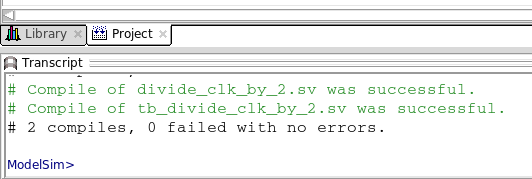
\includegraphics[scale=0.6]{ModelSim_tut_07}
\caption{Command prompt showing successful compilation.}
\label{Figure:Files_compiled2}
\end{figure}
%
% Compiled files2
%
\item \label{item:sim_step} The next step is to simulate our testbench.
On the top menu, select \textbf{Simulate} $\rightarrow$ \textbf{Start Simulation}. 
You should be prompted with a window as shown in \fref{Figure:Start_sim1}. 
%
% Start sim
%
\begin{figure}[!htb]
\centering
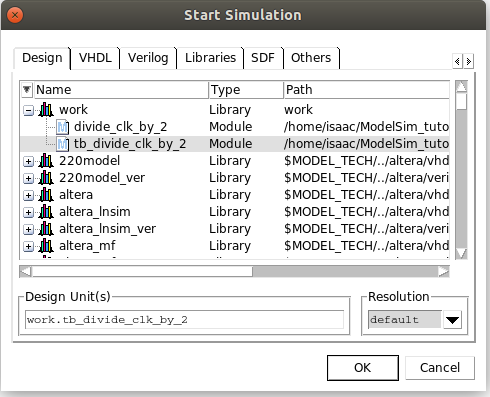
\includegraphics[scale=0.6]{ModelSim_tut_08a}
\caption{Start simulation.}
\label{Figure:Start_sim1}
\end{figure}
%
% Start sim
%
\newline
Click on the \textbf{+} sign next to \textbf{work}, select \SVtbdividefile and click \textbf{OK}. You should see something similar to \fref{Figure:Sim_env}.
%
% Sim env
%
\begin{figure}[!htb]
\centering
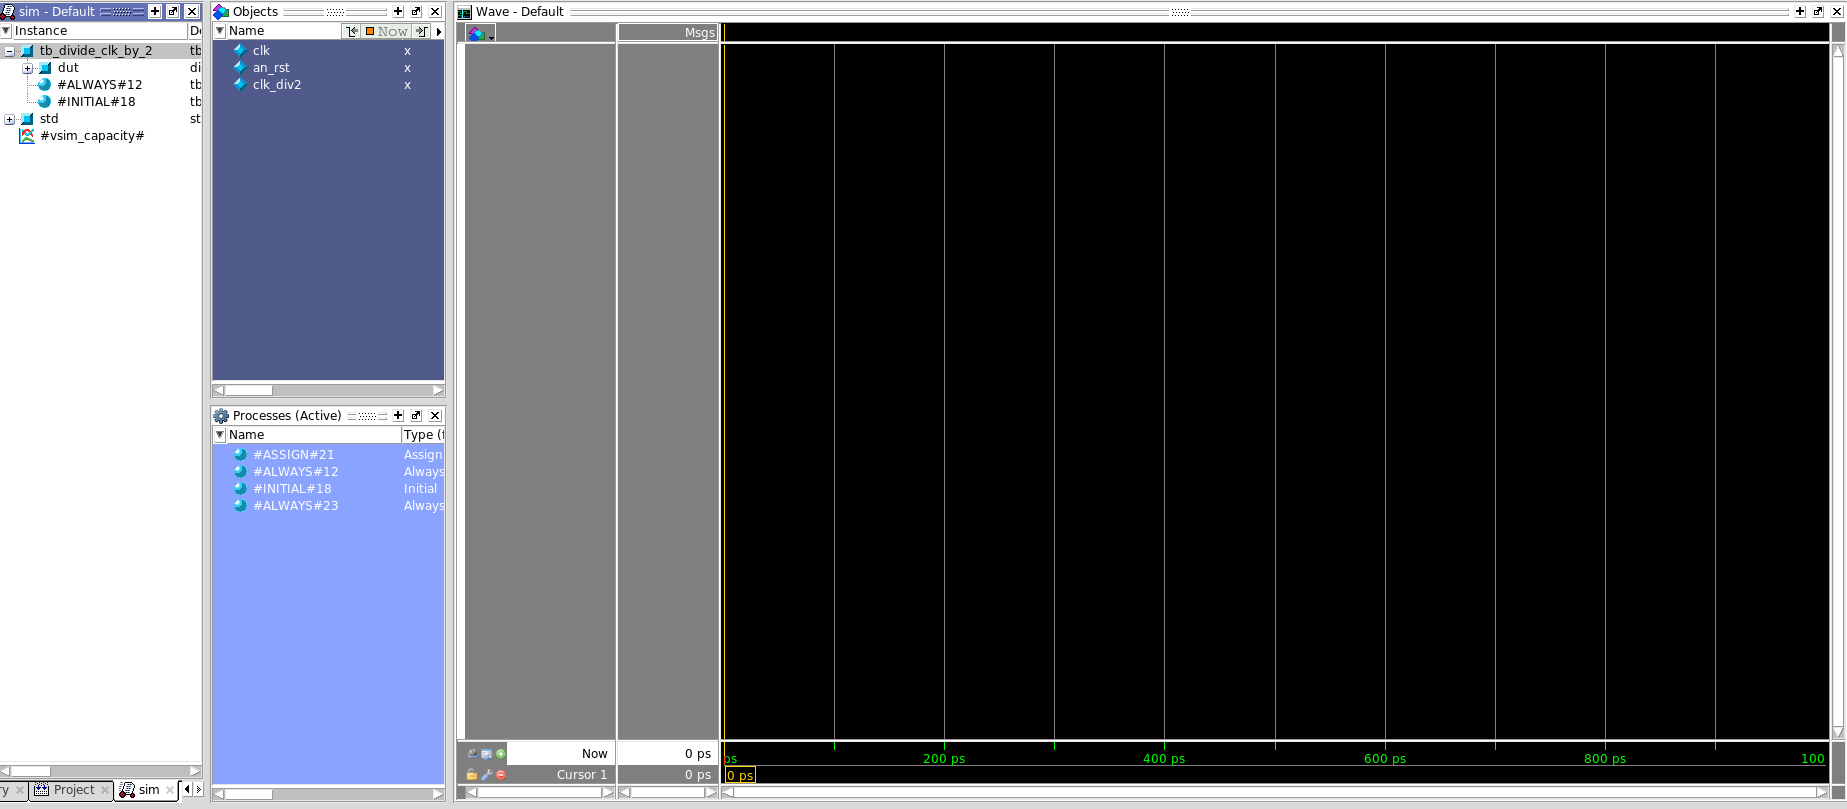
\includegraphics[width=\textwidth]{ModelSim_tut_09}
\caption{Simulation environment.}
\label{Figure:Sim_env}
\end{figure}
%
% Sim env
%
\newpage
\item In the \textbf{Objects} panel select all signals, right click and select \textbf{Add Wave} as shown in \fref{Figure:Adding_waves}.
%
% Adding waveforms
%
\begin{figure}[!htb]
\centering
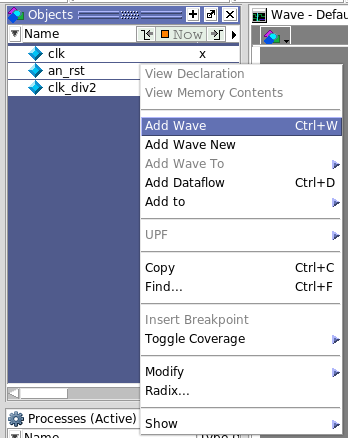
\includegraphics[scale=0.6]{ModelSim_tut_10}
\caption{Adding waveforms.}
\label{Figure:Adding_waves}
\end{figure}
%
% Adding waveforms
%
\newpage
Our testbench signals are now added to the \textbf{Wave} panel as shown in \fref{Figure:Signals_wave}.
%
% Waveforms added
%
\begin{figure}[!htb]
\centering
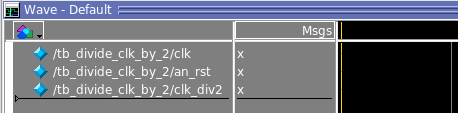
\includegraphics[scale=0.6]{ModelSim_tut_11}
\caption{Signals added to waveform panel.}
\label{Figure:Signals_wave}
\end{figure}
%
% Waveforms added
%
\item So far, we've compiled our source files, loaded our simulation environment and our testbench. 
However, we haven't actually started our simulation.
In order to start our simulation, on the top menu select \textbf{Simulation} $\rightarrow$ \textbf{Run} $\rightarrow$ \textbf{Run -All}. 
\ModelSim will perform the simulation and it should open the testbench file pointing to a \code{\$stop} construct as shown in \fref{Figure:Testbench_stop}. 
This is a control statement used in testbenches in order to prevent the simulator to continue with its simulation indefinitely. 
Go back to the waveform panel by clicking on \textbf{Wave} next to the name of the testbench, as shown in the lower left corner of \fref{Figure:Testbench_stop}.
%
% Waveforms added
%
\begin{figure}[!htb]
\centering
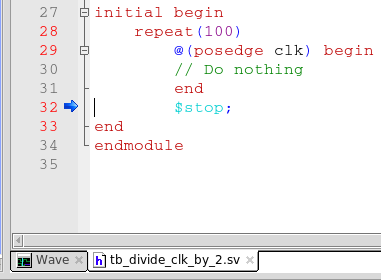
\includegraphics[scale=0.6]{ModelSim_tut_12}
\caption{\code{\$stop} construct in testbenches.}
\label{Figure:Testbench_stop}
\end{figure}
\newpage
\item In order to properly view our waveforms, we must zoom out. We can do this by either clicking on the icon to the right to the magnifier with the - sign, or by simply clicking anywhere in the wave panel and pressing \textbf{F}, as shown in \fref{Figure:Zoom_wave}.
%
% Waveforms added
%
\begin{figure}[!htb]
\centering
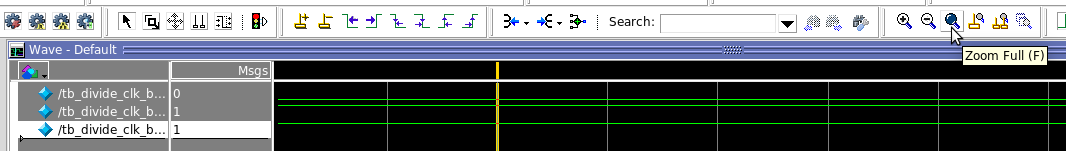
\includegraphics[width=\textwidth]{ModelSim_tut_13}
\caption{Zooming out in wave panel.}
\label{Figure:Zoom_wave}
\end{figure}

You should be able to see waveforms for the entire simulation time as shown in \fref{Figure:Full_wave}.
%
% Waveforms added
%
\begin{figure}[!htb]
\centering
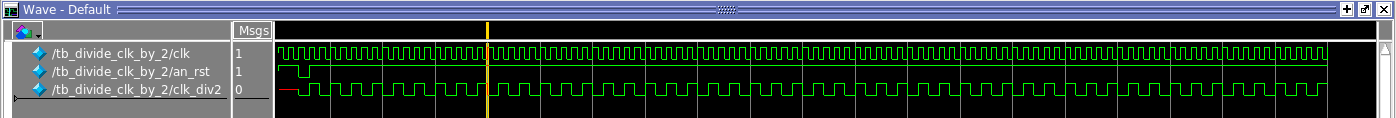
\includegraphics[width=\textwidth]{ModelSim_tut_14}
\caption{Full waveform view.}
\label{Figure:Full_wave}
\end{figure}
%
% Waveforms added
%

Use the magnifiers in order to zoom in and zoom out as you please.
It is also possible to zoom in using the middle click of the mouse. 
Moreover, there are defined shortcut keys for zooming in and out. 
Right click on the \textbf{wave} region and you can find out the different zoom shortcuts.

\item Hover over the icons shown in \fref{Figure:Sim_icons} in order to see different simulation run options.
Click on these buttons and identify what each of them does. 

\textbf{HINT:} You might have to \alertred{manually} stop the simulation by clicking on the red stop sign from \fref{Figure:Sim_icons}.

%
% Waveforms added
%
\begin{figure}[!htb]
\centering

\includegraphics[scale=1]{ModelSim_tut_15}
\caption{Quick simulation buttons.}
\label{Figure:Sim_icons}
\end{figure}
%
% Waveforms added
%
\item Identify which button restarts the simulation. Click on it and when prompted with a confirmation dialogue box, click \textbf{OK}. 
How could you run the simulation again? 
What happens when you change the default simulation step and click on the \textbf{Run} button? 
In my case, the default simulation value is set to \code{100 ps}. 
However, this value might be different in your environment.
Play around with these buttons, as well as with the simulation step and make sure you understand what each of them does.

\item Close \ModelSim and open it again, it will automatically load your last project.
Try to run your last simulation starting from step \ref{item:sim_step} from above in order to reinforce what you have learned.
\item Once you are familiar with how to launch and restart a simulation, finish your simulation by selecting \textbf{Simulate} $\rightarrow$ \textbf{End Simulation} $\rightarrow$ \textbf{Yes}.
\item You have finished the \ModelSim part of the tutorial. 
You may now proceed to the \ModelSim exercise in \sref{sec:ModelSim_exercise}.
\end{enumerate}

\subsection{\ModelSim exercise}\label{sec:ModelSim_exercise}
\begin{enumerate}
\item Create a new \ModelSim project using the file \SVcounterfile and its testbench \\\SVtbcounterfile.
\item Once you create the project, compile the files. 
\alertred{There should be syntax errors!} 
\item Debug the errors by double-clicking on the error messages that will appear in red font in the command prompt inside \ModelSim. 
A window should be opened with information about which line of code contains the error and a hint on how to fix it.
\item Fix all the errors until all error messages are gone.
\item Continue with the steps necessary in order to simulate the design.
\item Zoom in to a relevant time window in order to properly observe the waveforms.
%\item Take a screenshot of the waveforms and save it for your deliverables as stated in \sref{sec:Deliverables}.\label{item:ModelSim_Waveforms_3bits}
\item Analyse the code in both \SVcounterfile and its testbench \\\SVtbcounterfile and answer the questions embedded in the code comments.
\item The provided code models a 3-bit counter. 
Modify your file(s) in order to simulate an 8-bit counter. 
%Take a screenshot of your simulated waveforms and save it for your deliverables as stated in \sref{sec:Deliverables}.\label{item:ModelSim_Waveforms_8bits}
\item You may now proceed to \sref{sec:Quartus_project}.
\end{enumerate}

\newpage
% ======================================
% QUARTUS PROJECT
% ======================================
\section{\Quartus project}\label{sec:Quartus_project}
This section reinforces the steps necessary in order to create a \Quartus project and synthesize a design
If you are confident enough, you may skip \sref{sec:Quartus_tutorial} and go straight to the exercise in \sref{sec:Quartus_exercise}.

\subsection{Tutorial Instructions}\label{sec:Quartus_tutorial}
For this part of the tutorial, please use the source file \SVdividefile.
\begin{enumerate}
\item Open \Quartus.
\item Select \textbf{New Project Wizard} from the menu, as shown in \fref{Figure:Quartus_project_wizard}.
  %
  %  Project wizard
  %
  \begin{figure}[!hptb]
    \centering
    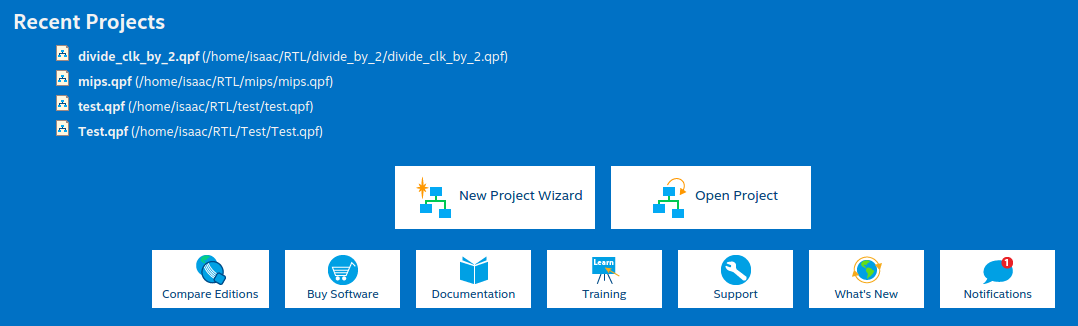
\includegraphics[width=\textwidth]{Quartus_tut_01_project_wizard}
    \caption{Project wizard.}
    \label{Figure:Quartus_project_wizard}
  \end{figure}
\newpage
\item When prompted with the \textbf{Introduction} window, click \textbf{Next} as shown in \fref{Figure:Quartus_project_wizard_intro}.
  %
  %  Project intro
  %
  \begin{figure}[!hptb]
    \centering
      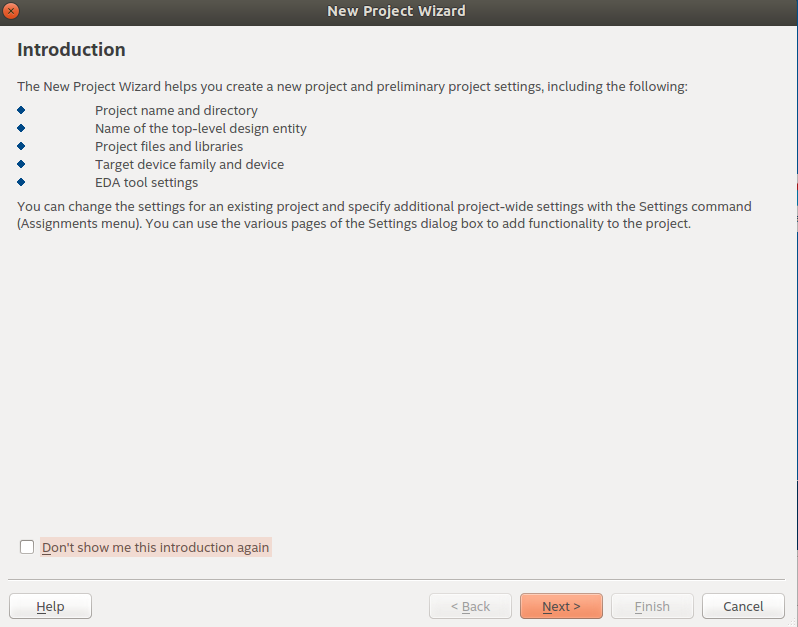
\includegraphics[width=\textwidth]{Quartus_tut_03_project_wizard_intro}
    \caption{Project intro.}
    \label{Figure:Quartus_project_wizard_intro}
  \end{figure}
\newpage
\item Provide a name for the project and click \textbf{Next}.

\alertblue{Important:} \Quartus requires that the name given to the project is the same as the top-level \SV~module.
As a result of this, name the project \SVdividefile, as shown in \fref{Figure:Quartus_project_name}.
  %
  %  Project name
  %
  \begin{figure}[!hptb]
    \centering
    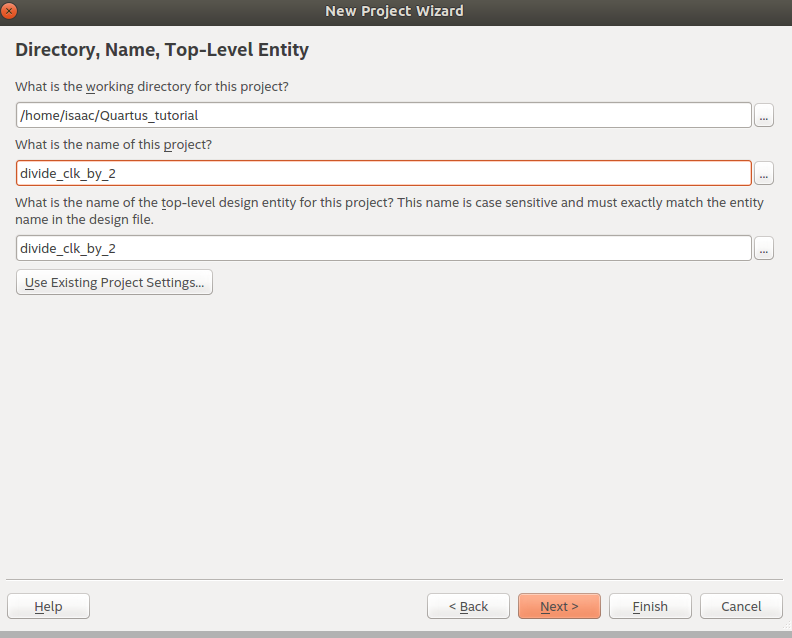
\includegraphics[width=\textwidth]{Quartus_tut_02_project_name}
    \caption{Project name.}
    \label{Figure:Quartus_project_name}
  \end{figure}
\newpage
\item Select \textbf{Empty project} as shown in \fref{Figure:Quartus_project_type} and click \textbf{Next}.        
    %
    %  Project type
    %
    \begin{figure}[!hptb]
      \centering
      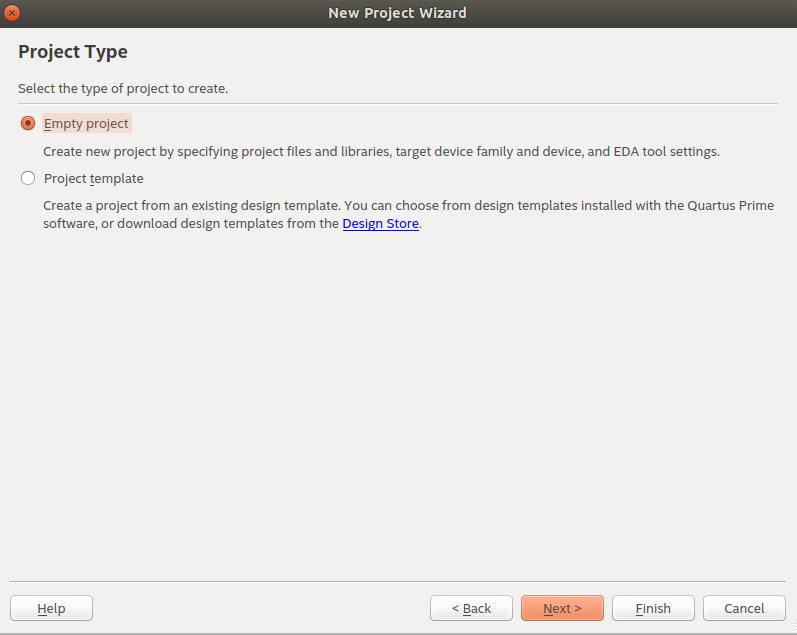
\includegraphics[width=\textwidth]{Quartus_tut_04_project_type}
      \caption{Project type.}
      \label{Figure:Quartus_project_type}
    \end{figure}
\newpage
\item When prompted to add files, browse to the location of the downloaded files and select \SVdividefile, as shown in \fref{Figure:Quartus_add_files}. 
Notice that testbenches are not synthesizable, as a result of this, we can simply omit our testbench.    
    %
    %  Adding files
    %
    \begin{figure}[!hptb]
      \centering
      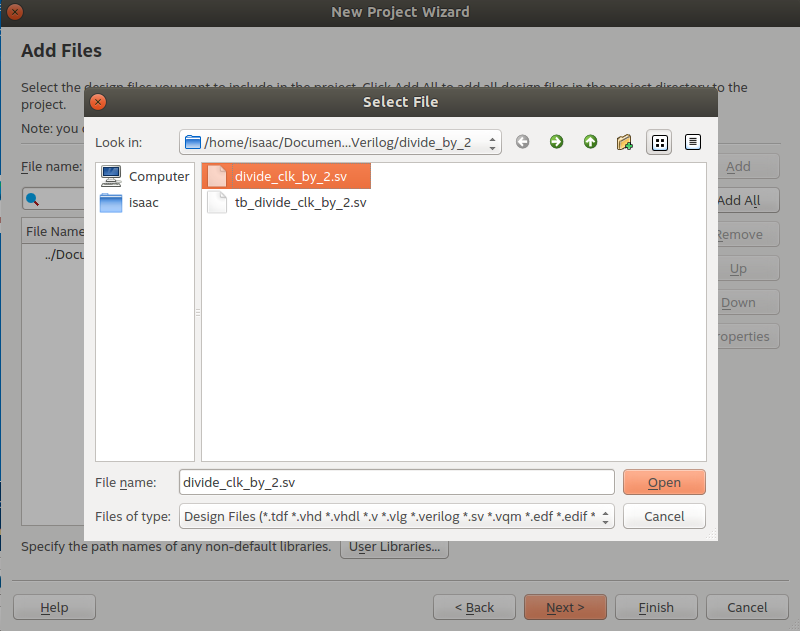
\includegraphics[width=\textwidth]{Quartus_tut_05_add_files}
      \caption{Adding files.}
      \label{Figure:Quartus_add_files}
    \end{figure}
\newpage
\item \Quartus allows us to select our target device, \ie, our target \ac{FPGA}. 
For this tutorial, we can simply click on \textbf{Next} in order to select the default device, as shown in \fref{Figure:Quartus_device}.
    %
    %  Quartus device
    %
    \begin{figure}[!hptb]
      \centering
      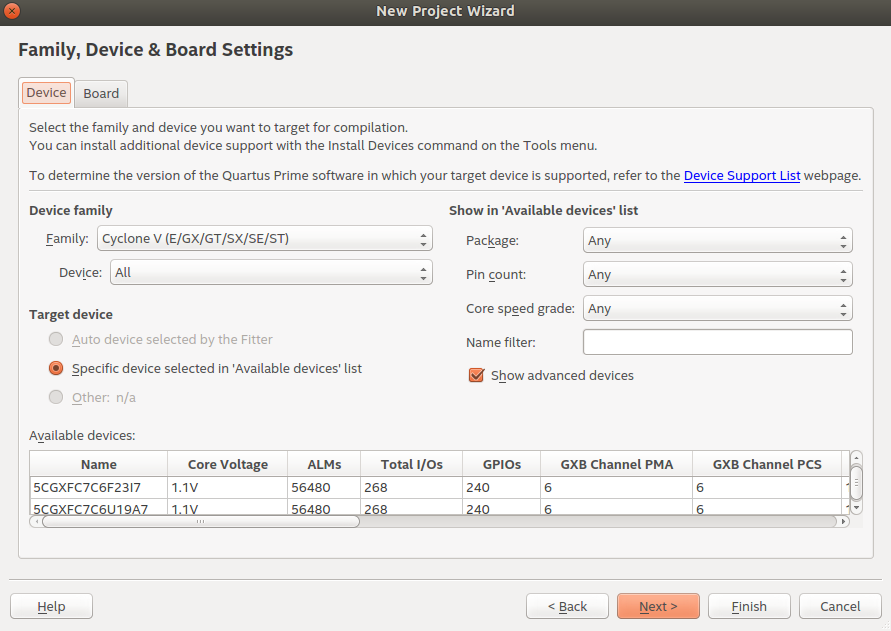
\includegraphics[width=\textwidth]{Quartus_tut_06_device}
      \caption{Selecting device.}
      \label{Figure:Quartus_device}
    \end{figure}
\newpage
\item The last step for creating a project is to select which other \ac{EDA} tools will be used. 
We can choose our simulation tool as well as some static check tools for timing and signal integrity.
However, for this tutorial, and for the majority of the course, we can simply click on \textbf{Next} without specifying any of the \acp{EDA}, as shown in \fref{Figure:Quartus_EDA}.
    %
    %  EDA
    %
    \begin{figure}[!hptb]
      \centering
      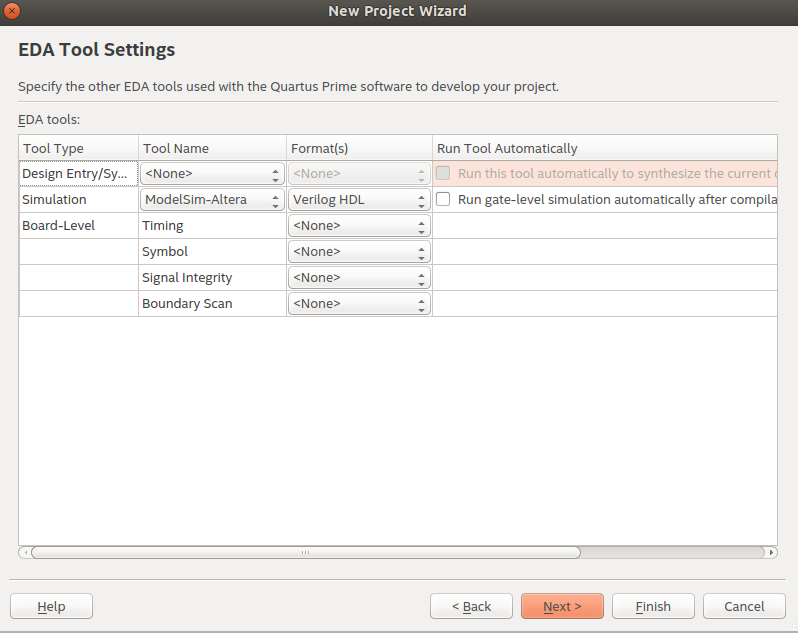
\includegraphics[width=\textwidth]{Quartus_tut_07_EDA}
      \caption{Selecting EDA.}
      \label{Figure:Quartus_EDA}
    \end{figure}
\newpage
\item Finally, \Quartus will prompt you with a summary of the project configuration. Click on \textbf{Finish} as shown in \fref{Figure:Quartus_summary}.    
    %
    %  Summary
    %
    \begin{figure}[!hptb]
      \centering
      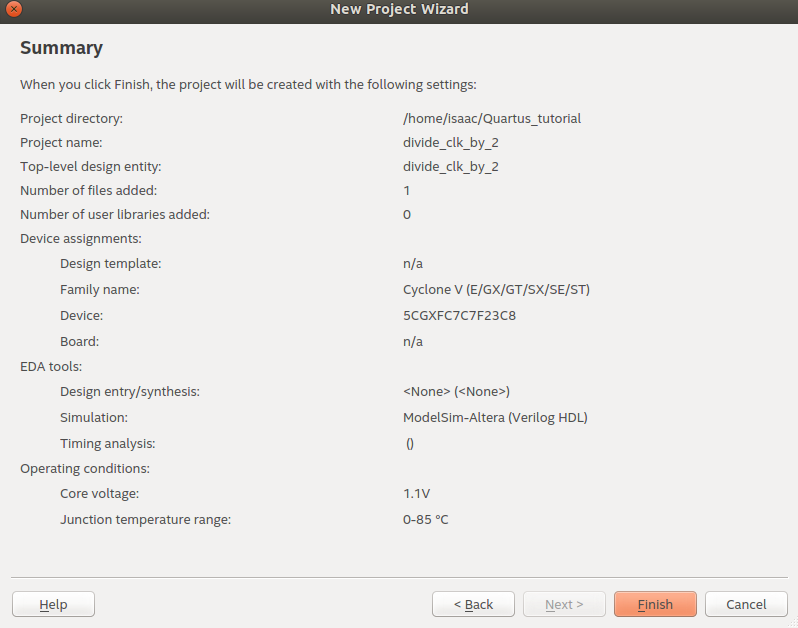
\includegraphics[width=\textwidth]{Quartus_tut_08_summary}
      \caption{Project summary.}
      \label{Figure:Quartus_summary}
    \end{figure}
\newpage
\item The project is now ready to be compiled. You should see something similar to \fref{Figure:Quartus_clean_project}. 
Here, the top part of the panel indicates the chosen device and the top-level unit to be compiled.
The bottom part shows the synthesis stages that \Quartus has performed.    
    %
    %  Project clean
    %
    \begin{figure}[!hptb]
      \centering
      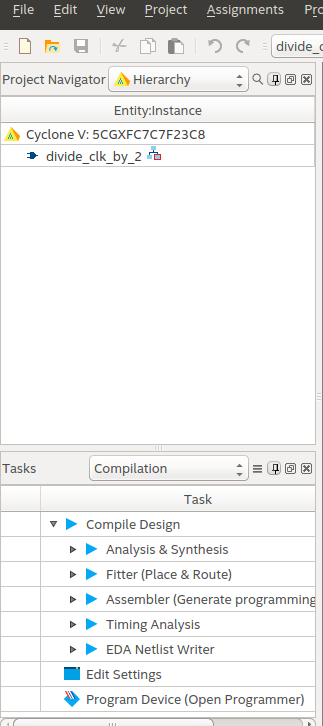
\includegraphics[scale=0.6]{Quartus_tut_09_clean_project}
      \caption{Project ready.}
      \label{Figure:Quartus_clean_project}
    \end{figure}
\newpage
\item The next step is to perform synthesis. Double click on the blue triangle/arrow next to \textbf{Compile Design}.
\Quartus should start the synthesis process and you should see some progress bars constantly updating.
This process can take several seconds or even minutes, depending on the computing power of your computer.    

\Quartus indicates that a design has been successfully synthesized by using green check marks next to each stage, as shown in \fref{Figure:Quartus_compilation}.
\Quartus will also show a summary in a new panel.
If a synthesis stage did not meet our constrains, \Quartus will use a red font to point to the failing stage.
In this case, you should see that we didn't meet the \alertred{Timing Analyzer} stage, as shown in the right side of \fref{Figure:Quartus_compilation}.
This is expected since we didn't specify any timing constrain.
Despite this, \Quartus was able to synthesise our design.
    %
    %  Quartus compilation
    %
    \begin{figure}[!hptb]
      \centering
      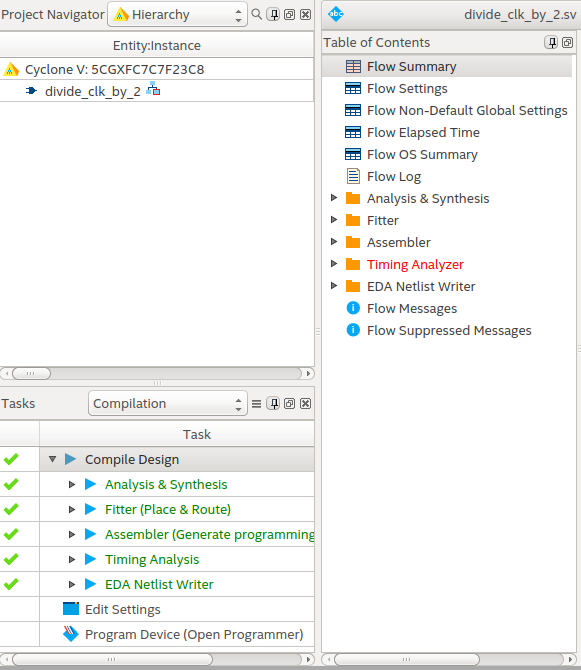
\includegraphics[scale=0.6]{Quartus_tut_10_compilation}
      \caption{Compiled project.}
      \label{Figure:Quartus_compilation}
    \end{figure}
\newpage
\item The next step is to have a look at the inferred \ac{RTL}. From the top menu, select \textbf{Tools} $\rightarrow$ \textbf{Netlist Viewers} $\rightarrow$ \textbf{RTL Viewer}, as shown in \fref{Figure:Quartus_rtl_menu}.
    %
    %  Project wizard
    %
    \begin{figure}[!hptb]
      \centering
      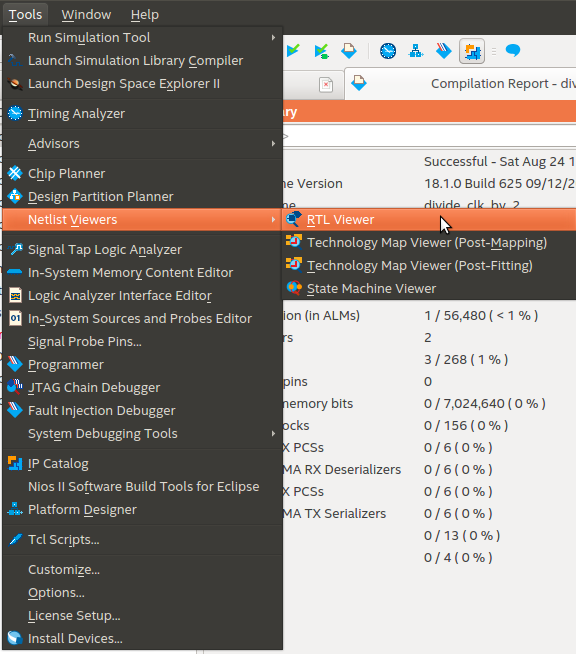
\includegraphics[scale=0.6]{Quartus_tut_11_rtl_menu}
      \caption{RTL view menu.}
      \label{Figure:Quartus_rtl_menu}
    \end{figure}
\item You should see something similar to \fref{Figure:Quartus_rtl}. 
Here, \fref{Figure:Quartus_rtl} shows how \Quartus logically interprets our \SV design.
    %
    %  Project wizard
    %
    \begin{figure}[!hptb]
      \centering
      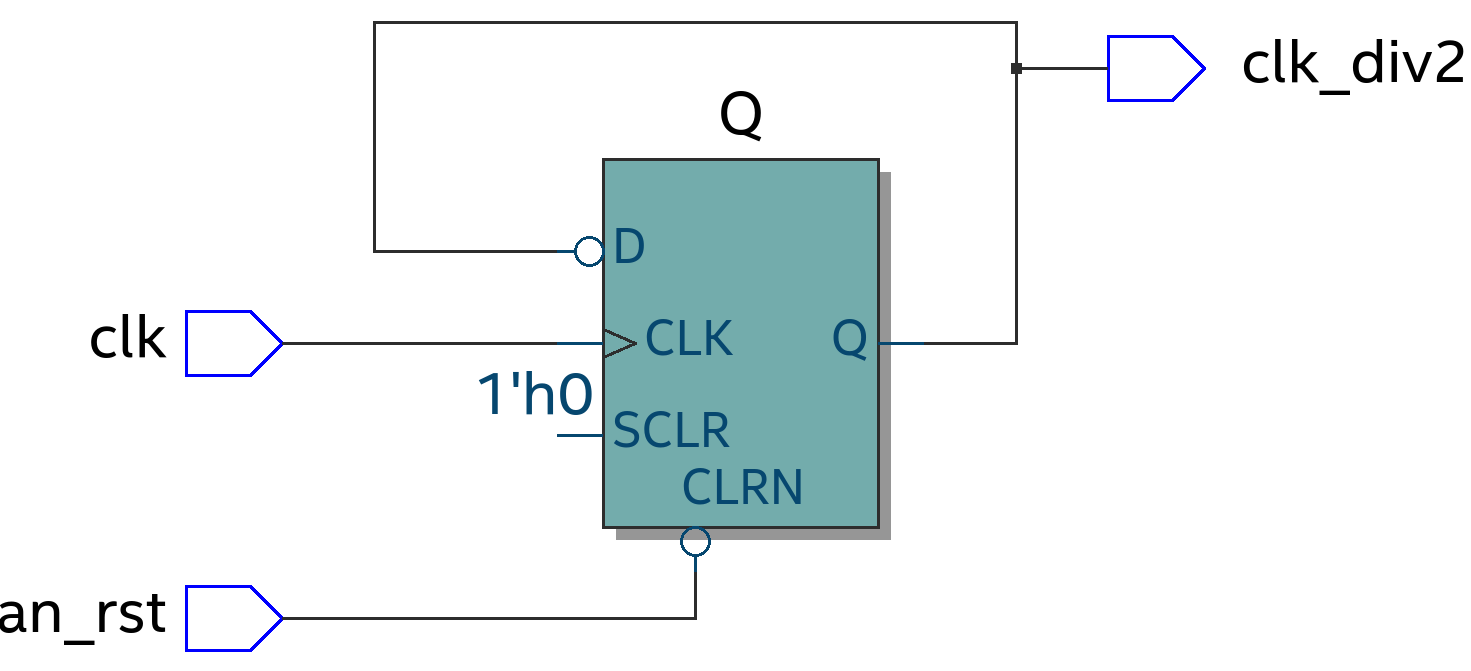
\includegraphics[scale=0.2]{Quartus_tut_12_rtl}
      \caption{RTL view.}
      \label{Figure:Quartus_rtl}
    \end{figure}
\item You may now close \Quartus and conclude the \Quartus part of this tutorial.
\item You may now proceed to the \Quartus exercise part of the tutorial in \sref{sec:Quartus_exercise}.   
\end{enumerate}

\subsection{\Quartus exercise}\label{sec:Quartus_exercise}
\begin{enumerate}
\item Create a new \Quartus project using the file \SVcounterfile.
\item Modify \SVcounterfile in order to synthesise a 6-bit counter.
\item Compile and synthesize the design. 
%\item Take a screenshot of the generated \ac{RTL} and save it for your deliverables as stated in \sref{sec:Deliverables}.\label{item:Quartus_RTL}
\item \alertdarkgreen{Congratulations!} You have finished this tutorial.
\end{enumerate}

%\section{Deliverables and Submission instructions}\label{sec:Deliverables}
%Prepare a single \code{zip} file containing the following. 
%\begin{enumerate}
%  \item Screenshots of your \ModelSim waveforms from steps \ref{item:ModelSim_Waveforms_3bits} and \ref{item:ModelSim_Waveforms_8bits} in \sref{sec:ModelSim_exercise}.
%  \item A screenshot of the generated \ac{RTL} for the 6-bit counter in \Quartus from step \ref{item:Quartus_RTL} in \sref{sec:Quartus_exercise}.
%  \item Your corrected versions of the source files \SVcounterfile and \SVtbcounterfile.
%\end{enumerate}

%Submit your assignment through Canvas before \deadline. 

\end{document}